%license:BSD-3-Clause
%copyright-holders:Michele Maione
%============================================================
%
%	Piattaforma di cloud gaming per giochi arcade
%
%============================================================

\chapter{Prestazioni} \label{cap:cap4}
%Si mostra il progetto dal punto di vista sperimentale, le cose materialmente realizzate. In questa sezione si mostrano le attività sperimentali svolte, si illustra il funzionamento del sistema (a grandi linee) e si spiegano i risultati ottenuti con la loro valutazione critica. Bisogna introdurre dati sulla complessità degli algoritmi e valutare l'efficienza del sistema.
Questo capitolo analizza le prestazioni del progetto relativamente ai tre difetti intrinseci del cloud gaming: riduzione della qualità audio-video, bit-rate richiesto e il problema della latenza.



\section{Qualità audio-video}
Nell'ambito videoludico la qualità audiovisiva (soprattutto la visiva) influisce sulla qualità generale percepita dall'utente, per questo nel cloud gaming è necessario garantire un livello di qualità quasi identico alla versione in locale. Lo streaming a bit-rate bassi è possibile preservando la qualità percepita ed è particolarmente adatto per l'utilizzo in reti mobili\footnote{Con l'utilizzo di tariffe flat per reti mobili. Solitamente sono abbonamenti solo dati per tablet e smartphone.} e WLAN \parencite{VideoAndMultimediaTransmissionsOverCellularNetworks}.



\subsection{Video}
Qualsiasi elaborazione applicata ad un'immagine può causare la perdita di qualità. La qualità dell'immagine si riferisce al modo in cui viene riprodotta la scena ripresa (o quella generata digitalmente) e può essere descritta dal degradarsi di alcune caratteristiche tra cui: nitidezza, gamma dinamica, fusione dei colori, contrasto, sfocatura, ecc\dots. I metodi di valutazione della qualità dell'immagine possono essere suddivisi in metodi oggettivi e soggettivi. I metodi oggettivi si basano su confronti utilizzando criteri numerici espliciti. L'errore quadratico medio (MSE), il \textit{peak signal-to-noise ratio} (PSNR) e la \textit{structural similarity index measure} (SSIM) sono esempi di misure di qualità utilizzate nell'analisi delle immagini \parencite{relationship_PSNR_and_SSI}.



\subsubsection{Peak signal-to-noise ratio}
Il PSNR è comunemente usato come misura della qualità della compressione e della riduzione del rumore nelle immagini digitali a scala di grigi. Esistono diversi approcci per calcolare il PSNR delle immagini a colori, ad esempio (il più semplice) utilizzando immagini in formato YCbCr e calcolando il PSNR solo sul canale della luminanza. Il PSNR è espresso solitamente in decibel con valori tipici per la compressione video per lo streaming tra $20$ \si{dB} e $25$ \si{dB} \parencite{ThomosN2006OtoJ} e si calcola utilizzando l'Eq. \ref{eq:PSNR} con $MSE(f,g)$ l'errore quadratico medio e $L = 255$ l'intervallo dinamico \parencite{AnewcombinedPSNRforobjectivevideoqualityassessment}.

\begin{equation} \label{eq:PSNR}
	PSNR(f,g)=10 \log_{10}  \frac{L^2}{MSE(f,g)}	
\end{equation}

\begin{figure}[H]
	\centering
	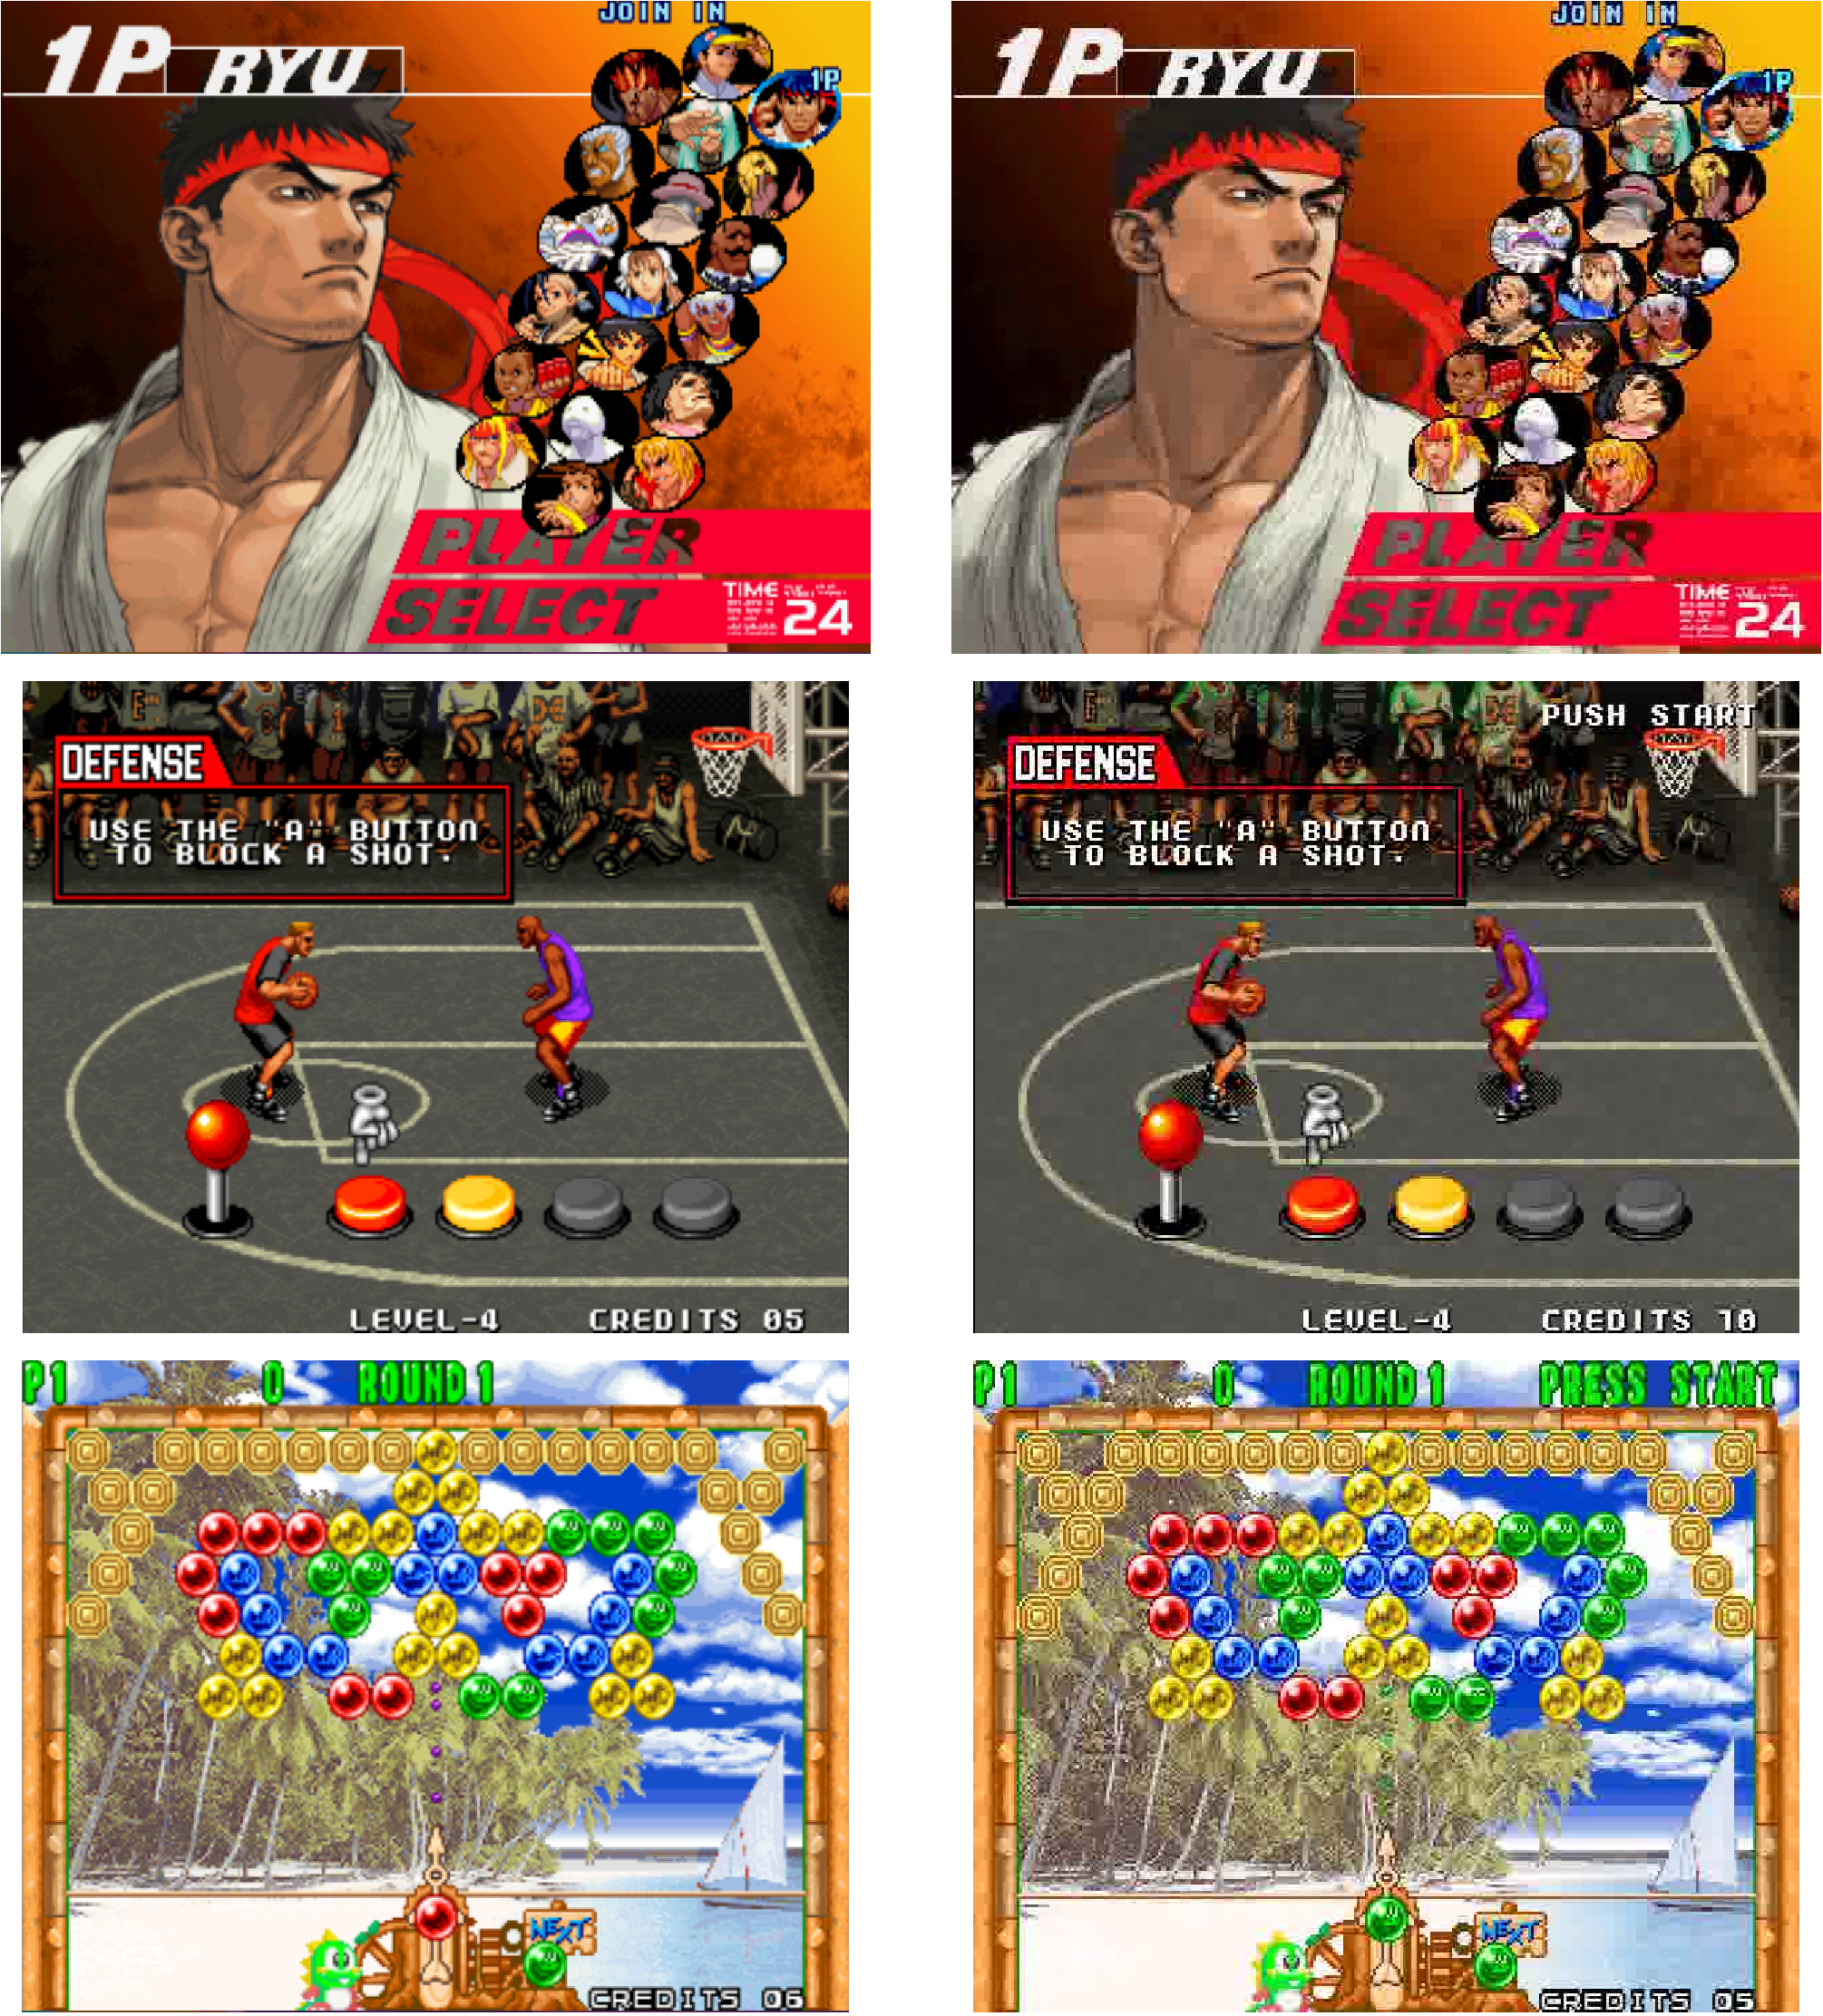
\includegraphics[width=\linewidth]{immagini/BMP_MPEG_compare}
	\caption{Alcuni frame d'esempio: a sinistra i frame renderizzati dal MAME (RGBA), a destra i frame codificati in \textit{MPEG-1}. © Capcom, Data East, Taito}
	\label{fig:BMP_MPEG_compare}
\end{figure}



\subsubsection{Structural Similarity Index Measure}
SSIM è un metodo per predirre la qualità percepità nelle immagini digitali. Invece di utilizzare i tradizionali metodi di somma degli errori, SSIM è progettato modellando qualsiasi distorsione dell'immagine come una combinazione di tre fattori: la perdita di correlazione, la distorsione della luminanza e la distorsione del contrasto. L'indice SSIM è un valore decimale compreso tra $0$ e $1$ e si calcola utilizzando l'Eq. \ref{eq:SSIM} con \parencite{relationship_PSNR_and_SSI}:

\begin{itemize}
	\item $k_1 = 0,01$ e $k_2 = 0,03$ costanti;
	\item $L = 255$ l'intervallo dinamico;
	\item $c_1 = (k_1 L)^2$, $c_2 = (k_2 L)^2$ e $c_3 = c_2/2$ variabili di stabilizzazione della divisione;
	\item $l(f,g)$ funzione di comparazione della luminanza tra le medie $\mu_f$ e $\mu_g$;
	\item $c(f,g)$ funzione di comparazione del contrasto tra le deviazioni standard $\sigma_f$ e $\sigma_g$;
	\item $s(f,g)$ funzione di comparazione della struttura che misura il coefficiente di correlazione; $\sigma_{fg}$ è la covarianza tra $f$ e $g$.
\end{itemize}

\begin{equation} \label{eq:SSIM}
	\begin{matrix*}[l]
		SSIM(f,g) =  l(f,g) c(f,g) s(f,g) & l(f,g)= \frac{2 \mu_f \mu_g  + C_1}{\mu_f^2 \mu_g^2  + C_1} \\
		c(f,g)= \frac{2 \sigma_f \sigma_g  + C_2}{\sigma_f^2 + \sigma_g^2  + C_2} & s(f,g)= \frac{\sigma_{fg}+C_3}{\sigma_f \sigma_g + C_3}
	\end{matrix*}
\end{equation}



\subsubsection{Risultati ottenuti}
Tramite lo script in Lis. \ref{lst:PyPSNR_SSIM} è stata calcolata la qualità video per la codifica \textit{MPEG-1 Video} che ha dato come risultati un valore di PSNR di $27,703$ \si{dB} e un indice SSIM del $89,9\%$. Alcune immagini d'esempio del risultato ottenuto sono visibili in Fig. \ref{fig:BMP_MPEG_compare}.

\begin{lstlisting}[language=Python, caption=Script Python per il calcolo di PSNR e SSIM, label={lst:PyPSNR_SSIM}]
imgRGB = skimage.io.imread("frameRGB.bmp")
imgMPEG1 = skimage.io.imread("frameMPEG1.bmp")

PSNR = skimage.metrics.peak_signal_noise_ratio(imgRGB, imgMPEG1)

SSIM = skimage.metrics.structural_similarity(imgRGB, imgMPEG1,
	multichannel=True)
\end{lstlisting}



\subsection{Audio}
Lorem ipsum dolor sit amet, consectetur adipiscing elit, sed do eiusmod tempor incididunt ut labore et dolore magna aliqua. Ut enim ad minim veniam, quis nostrud exercitation ullamco laboris nisi ut aliquip ex ea commodo consequat. Duis aute irure dolor in reprehenderit in voluptate velit esse cillum dolore eu fugiat nulla pariatur. Excepteur sint occaecat cupidatat non proident, sunt in culpa qui officia deserunt mollit anim id est laborum.



\subsubsection{Total Harmonic Distortion}
Lorem ipsum dolor sit amet, consectetur adipiscing elit, sed do eiusmod tempor incididunt ut labore et dolore magna aliqua. Ut enim ad minim veniam, quis nostrud exercitation ullamco laboris nisi ut aliquip ex ea commodo consequat. Duis aute irure dolor in reprehenderit in voluptate velit esse cillum dolore eu fugiat nulla pariatur. Excepteur sint occaecat cupidatat non proident, sunt in culpa qui officia deserunt mollit anim id est laborum.




\section{Bit-rate}
Il cloud gaming effettua lo streaming in tempo reale lorem ipsum dolor sit amet, consectetur adipiscing elit, sed do eiusmod tempor incididunt ut labore et dolore magna aliqua. Ut enim ad minim veniam, quis nostrud exercitation ullamco laboris nisi ut aliquip ex ea commodo consequat. Duis aute irure dolor in reprehenderit in voluptate velit esse cillum dolore eu fugiat nulla pariatur. Excepteur sint occaecat cupidatat non proident, sunt in culpa qui officia deserunt mollit anim id est laborum \parencite{Network_Analysis_of_the_Sony_Remote_Play_System}.

Lorem ipsum dolor sit amet, consectetur adipiscing elit, sed do eiusmod tempor incididunt ut labore et dolore magna aliqua. Ut enim ad minim veniam, quis nostrud exercitation ullamco laboris nisi ut aliquip ex ea commodo consequat. Duis aute irure dolor in reprehenderit in voluptate velit esse cillum dolore eu fugiat nulla pariatur. Excepteur sint occaecat cupidatat non proident, sunt in culpa qui officia deserunt mollit anim id est laborum.
\parencite{StreamingMobileCloudGamingVideoOverTCPWithAdaptiveSourceFECCoding}




\section{Latenza} \label{sec:cap4_Latenza}
Per quanto riguarda la latenza è un problema che non può essere eliminato nel cloud gaming perché le fasi di un videogioco sono: ricezione input, esecuzione, rendering, display; mentre nel caso del cloud gaming si aggiungono: invio al server dell'input utente, codifica audio-video, invio all'utente dello stream video, decodifica audio-video. Un leggero ritardo in un filmato su internet o in una videochiamata molto probabilmente passa inosservato, ma durante una partita la latenza può rendere il gioco ingiocabile, una tempistica di esempio è visibile in Fig. \ref{fig:latenzaCloudGaming}, fortunatamente il rapido sviluppo delle reti a banda larga hanno reso questo problema meno evidente e il cloud gaming una realtà \parencite{Cloud_Gaming_Architecture_and_Performance}.

\begin{figure}[H]
	\includegraphics[width=\linewidth]{immagini/latenzaCloudGaming.png}
	\caption{Latenza del videogioco: locale vs cloud gaming.}
	%Fonte: shadow.tech/blog/news/roadmap-cloud-gaming-without-latency
	\label{fig:latenzaCloudGaming}
\end{figure}

Come mostrato in tabella \ref{table:Ritardo_tollerato_per_tipo_di_gioco} lorem ipsum dolor sit amet, consectetur adipiscing elit, sed do eiusmod tempor incididunt ut labore et dolore magna aliqua. Ut enim ad minim veniam, quis nostrud exercitation ullamco laboris nisi ut aliquip ex ea commodo consequat. Duis aute irure dolor in reprehenderit in voluptate velit esse cillum dolore eu fugiat nulla pariatur. Excepteur sint occaecat cupidatat non proident, sunt in culpa qui officia deserunt mollit anim id est laborum \parencite{Cloud_Gaming_Architecture_and_Performance}.

\begin{table}[H]
	\centering
	\begin{tabular}{||l l r||}
		\hline
		Tipo di gioco & Prospettiva & Soglia di ritardo (ms) \\
		\hline\hline
		FPS & Prima persona & 100 \\
		\hline
		RPG & Terza persona & 500 \\
		\hline
		RTS & Onnipresente & 1000 \\
		\hline
	\end{tabular}

	\caption{Ritardo tollerato per tipo di gioco}
	\label{table:Ritardo_tollerato_per_tipo_di_gioco}
\end{table}